\section{Resultados e Discussões}%
\label{sec:resultados}%

Havendo sido decididos o escopo do minicurso e a temática do jogo a ser desenvolvido, os autores se dedicaram à implementação do jogo e à preparação do material de apoio para a aplicação daquele a turmas de graduação.

\subsection{Implementação do Jogo}

À luz do disposto, foi escolhida como temática um jogo a construção de uma vila, em que a cada \texttt{click} em uma ação o usuário realiza uma ação pré-definida.
A inicialmente disponibilizada é chamada de ``cortar madeira'', em que o usuário obtém uma cópia do recurso ``madeira''.
Ao adquirir o suficiente, ele pode executar a ação ``vender madeira''
o que remove uma unidade de ``madeira'' do inventário e adiciona uma porção equivalente de ``ouro''.

Outra mecânica do jogo é a geração automática de recursos. Esta característica é implementada através da ação de ``contratar trabalhadores'', o que exige uma unidade do recurso ``casa'' e certa porção de ``ouro''.
Uma vez contratados eles passam a fornecer um fluxo constante de ``madeira'' por segundo, o que permite ao jogador acumular recursos mesmo sem interação.

Cada recurso é representado por um componente \gls{html} chamado ``section''.
Já cada ação apresenta, dentro de sua seção, um elemento ``button'' que, ao ser clicado, executa a ação correspondente.
O uso de elementos semânticos do \gls{html} é uma prática recomendada para a construção de páginas acessíveis e bem estruturadas~\cite{whatwg:2025:html_standard_semantics}.
A \autoref{fig:interface} apresenta a interface do jogo em execução.

\begin{figure}[!htb]%
    \caption{\label{fig:interface}%
        Captura de tela do jogo em execução.%
    }%
    \centering%
    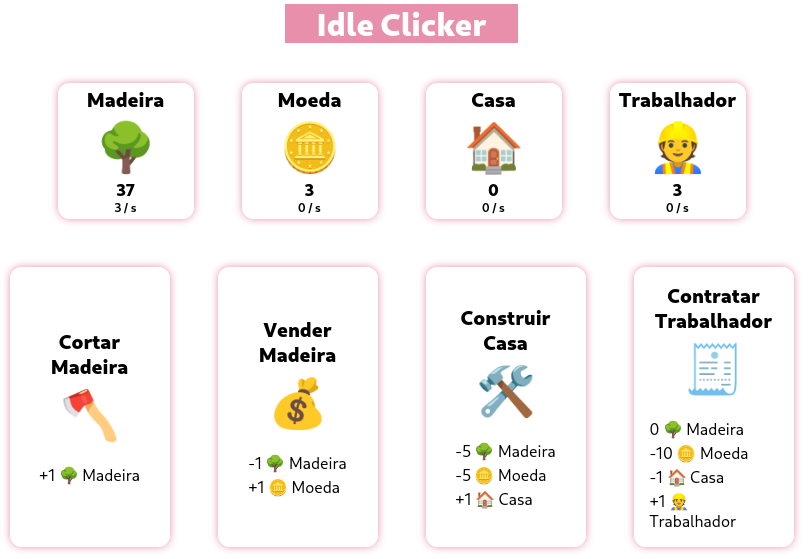
\includegraphics[width=0.75\textwidth]{imagens/interface.png}%
    \legend{\ComponenteFontePropria}%
\end{figure}

\subsection{Aplicação do Minicurso}

A fim de aplicar o minicurso, foi desenvolvido um material de apoio composto por slides que disponibilizam o código de forma progressiva.
Ele é divido em passos com comentários que visam a possibilitar o desenvolvimento do jogo por um iniciante interessado mesmo sem a presença de um instrutor.
Posteriormente, o material foi transformado em um livro digital disponibilizado publicamente~\cite{malosto:2024:comecando_no_react}, de forma que poder ser acessado por qualquer pessoa em qualquer tempo.
A \autoref{fig:livro} apresenta um trecho do livro digital.

\begin{figure}[!htb]%
    \caption{\label{fig:livro}%
        Trecho do livro digital de apoio ao minicurso, em que se apresenta o código-fonte do componente de exibição de um recurso.%
    }%
    \centering%
    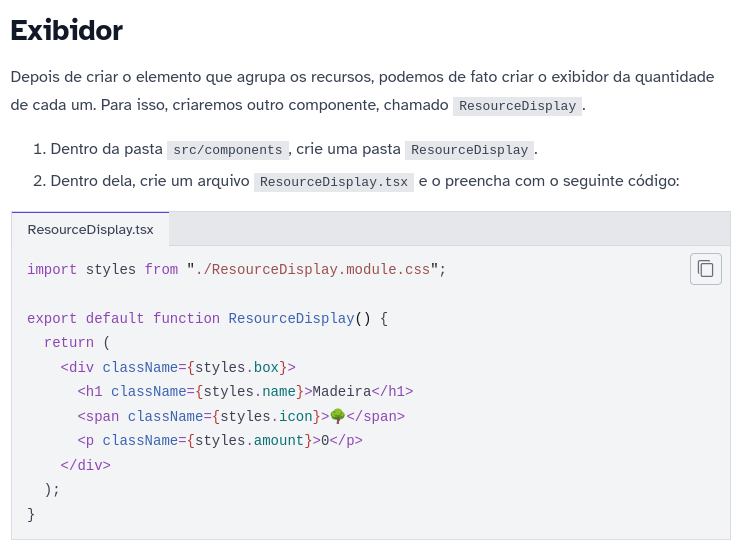
\includegraphics[width=0.75\textwidth]{imagens/livro.png}%
    \legend{\ComponenteFontePropria}%
\end{figure}

A primeira aplicação do minicurso ocorreu em 2022, durante a Semana do \gls{ice} na \gls{ufjf}.
Neste momento, ainda não havíamos incluído o \gls{ts} no escopo do curso.
Na ocasião, duas turmas contando com cerca de 40 pessoas foram montadas.
Aquela cujo horário permitiu um período de quatro horas teve a cobertura de todo o conteúdo planejado.
Já a outra, com apenas três horas disponíveis, não conseguiu chegar ao final do material, em que se implementa a geração automática de recursos.

Uma vez que o público-alvo se  tratava de discentes de cursos ligados ao \gls{dcc} da \gls{ufjf}, esperávamos que houvesse familiaridade com programação.
Entretanto, percebemos que nem todos os alunos estavam familiarizados especificamente com o desenvolvimento Web, uma vez que a temática apenas era de caráter obrigatório ao curso de \gls{bsi}.
O \gls{ice} se tornou ciente dessa necessidade, que foi exposta pelo feedback dos alunos quanto ao curso e quanto a outros projetos e disciplinas da universidade.
Dessa forma, o currículo dos cursos de \gls{bcc} passou a incluir uma disciplina focada em \gls{pw}.

Após o curso ser ministrado em diferentes eventos por dois anos consecutivos, identificamos a necessidade de evoluir o material.
Portanto, refizemos o código de referência e o material de apoio para utilizarem a linguagem \gls{ts}.
O objetivo dessa mudança é evitar erros comuns de desenvolvimento e facilitar a manutenção do código.
Também simplificamos tópicos que não eram essenciais para o aprendizado de React, a fim de garantir melhor aproveitamento do tempo disponível.

Em 2024, o minicurso contou com a presença de uma nova membro do GetSi atuando como monitora para auxiliar os alunos a resolver erros pontuais e acompanhar a apresentação.
Ainda que em outros anos recebemos ajuda semelhante de outros discentes, isto ocorria de forma casual e sem planejamento.
A presença de um monitor dedicado permitiu que os instrutores se concentrassem em apresentar o conteúdo, sem se preocupar com questões técnicas.
